\subsection{ALU Execution Pipeline}\label{sec:alu-exe-pip}

The ALU execution pipeline executes ALU and branch instructions (including \inst{CSRRW} instructions).
To sustain peak throughput for ALU instructions with back-to-back dependencies, the pipeline contains bypass logic and wakes up dependent instructions aggressively.

\subsubsection{Interface}

\begin{figure}
\begin{lstlisting}[caption={}]
interface AluExeInput;
  method RegsReady sbCons_lazyLookup(PhyRegs r);
  method Data rf_rd1(PhyRIndx rindx);
  method Data rf_rd2(PhyRIndx rindx);
  method Data csrf_rd(CSR csr);
  method Addr rob_getPC(InstTag t);
  method Addr rob_getPredPC(InstTag t);
  method Action rob_setExecuted(InstTag t, Maybe#(Data) csrData, ControlFlow cf);
  method Action fetch_train_predictors(FetchTrainBP train);
  method Action setRegReadyAggr(PhyRIndx dst);
  interface Vector#(2, SendBypass) sendBypass;
  method Action writeRegFile(PhyRIndx dst, Data data);
  method Action redirect(Addr new_pc, SpecTag spec_tag, InstTag inst_tag);
  method Action correctSpec(SpecTag t);
  method Bool doStats;
endinterface
interface AluExePipeline;
  interface Vector#(TMul#(2, AluExeNum), RecvBypass) recvBypass;
  interface ReservationStationAlu rsAluIfc;
  interface SpeculationUpdate specUpdate;
  method Data getPerf(ExeStagePerfType t);
endinterface
module mkAluExePipeline#(AluExeInput inIfc)(AluExePipeline);
  // implementation
endmodule
\end{lstlisting}
\caption{Interface of ALU execution pipeline}\label{fig:alu-exe-pipe-ifc}
\end{figure}

Figure~\ref{fig:alu-exe-pipe-ifc} shows the interface of the ALU execution pipeline.
Interface \code{AluExeInput} is the input argument to the module.
It contains the following fields:
\begin{itemize}
    \item Methods \code{sbCons\_lazyLookup}, \code{rf\_rd1} and \code{rf\_rd2}: read the conservative scoreboard and physical register file.
    \item Method \code{csrf\_rf}: reads the CSR register file.
    This is called by the module in case of the \inst{CSRRW} instruction.
    \item Methods \code{rob\_getPC} and \code{rob\_getPredPC}: retrieve PC and predicted PC (by the fetch pipeline), respectively, from the corresponding ROB entry.
    \item Method \code{rob\_setExecuted}: sets the ROB entry as executed, so the instruction can be committed if it is the oldest in ROB.
    \item Method \code{fetch\_train\_predictors}: trains the branch predictors in the fetch pipeline.
    \item Method \code{setRegReadyAggr}: wakes up dependent instructions in all the reservation stations, and sets the aggressive scoreboard.
    \item Subinterface \code{sendBypass}: is called by the module to send out data forwardings to other execution pipelines and itself.
    \item Method \code{writeRegFile}: writes the physical register file.
    \item Method \code{redirect}: redirects the fetch pipeline, increments the epoch in the epoch manager, and calls the global speculation updater to kill wrong-path instructions (i.e., call the \code{incorrectSpeculation} method of every module).
    This method is called by the ALU execution pipeline in case of branch mispreditions.
    \item Method \code{correctSpec}: calls the global speculation updater to release a speculation tag (i.e., call the \code{correctSpeculation} method of every module).
    This method is called by the ALU execution pipeline in case of correct branch preditions.
    \item Method \code{doStats}: returns whether performance counters should be incremented or not.
\end{itemize}
The module interface \code{AluExePipeline} contains the following fields:
\begin{itemize}
    \item Subinterface \code{recvBypass}: receives the data forwardings sent by other execution pipelines and itself.
    That is, interface \code{sendBypass} in the module argument will call this interface.
    \item Subinterface \code{rsAluIfc}: returns the reservation station inside the pipeline.
    \item Subinterface \code{specUpdate}: manipulates speculative states (Section~\ref{sec:specupdate}).
    \item Method \code{getPerf}: is for querying performance counters.
\end{itemize}

\subsubsection{Implementation}

\begin{figure}
    \centering
    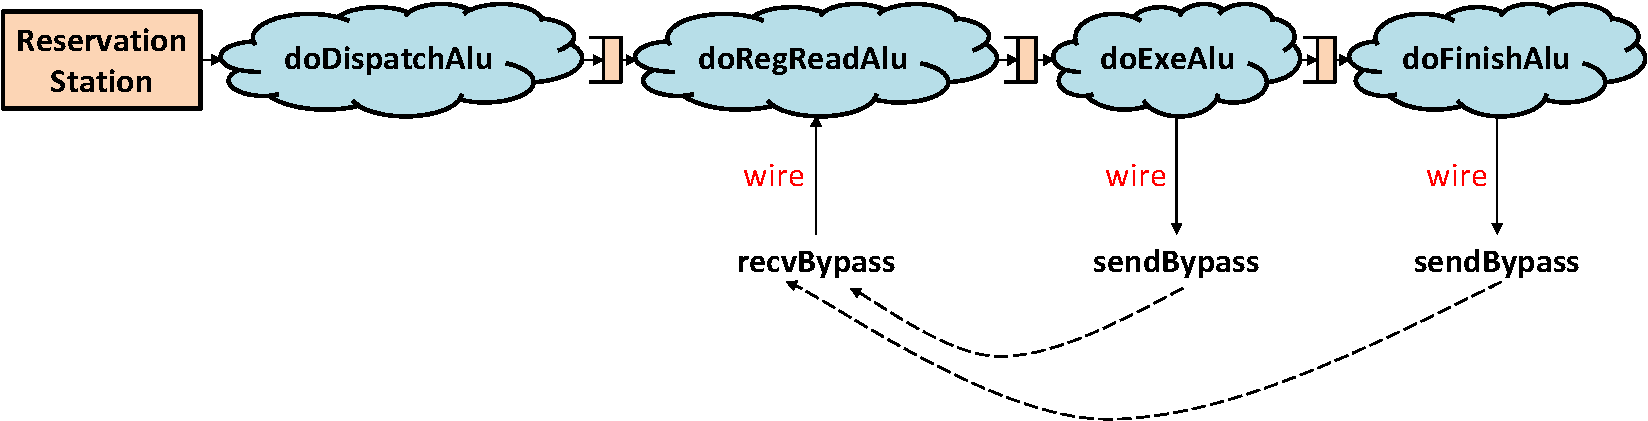
\includegraphics[width=\columnwidth]{fig/alu_exe_crop.pdf}
    \caption{Internal implementation of ALU execution pipeline}\label{fig:alu-exe-pipe-impl}
\end{figure}

Figure~\ref{fig:alu-exe-pipe-impl} shows the internal implementation of the ALU execution pipeline.
All the pipeline stages are connected by speculation FIFOs (Section~\ref{sec:specfifo}).
Sending and receiving data forwardings are done by using \emph{wires}.
The pipeline contains the following four internal rules:
\begin{itemize}
    \item Rule \code{doDispatchAlu}: retrieves a ready instruction from the reservation station.
    \item Rule \code{doRegReadAlu}: first checks data forwardings and then checks the conservative scoreboard and physical register if forwarding is not available.
    The rule will not fire if a source register is not available.
    \item Rule \code{doExeAlu}: executes the instruction by performing the ALU operation or calculating the next PC.
    The result for the destination register is sent to a wire which will be exported as the \code{sendBypass} interface.
    \item Rule \code{doFinishAlu}: marks the ROB entry as executed, and sends data forwarding to a wire.
    In case of a branch, either \code{correctSpec} or \code{redirect} will be called.
    To avoid conflict with other rules, this rule is split into two based on whether a branch is mispredicted or not.
    The common case without mispredictions will not conflict with other common rules.
\end{itemize}

\subsubsection{Future Improvement}
We should remove the wires for data forwardings.
An alternative way is to add a bypass method to every pipeline-stage FIFO, and sending data forwardings is directly calling this method of all the relevant pipeline-stage FIFOs.

\subsubsection{Source Code}
See module \code{mkAluExePipeline} in \code{//procs/RV64G\_OOO/AluExePipeline.bsv}.
